% Created by tikzDevice version 0.7.0 on 2015-04-23 16:55:32
% !TEX encoding = UTF-8 Unicode
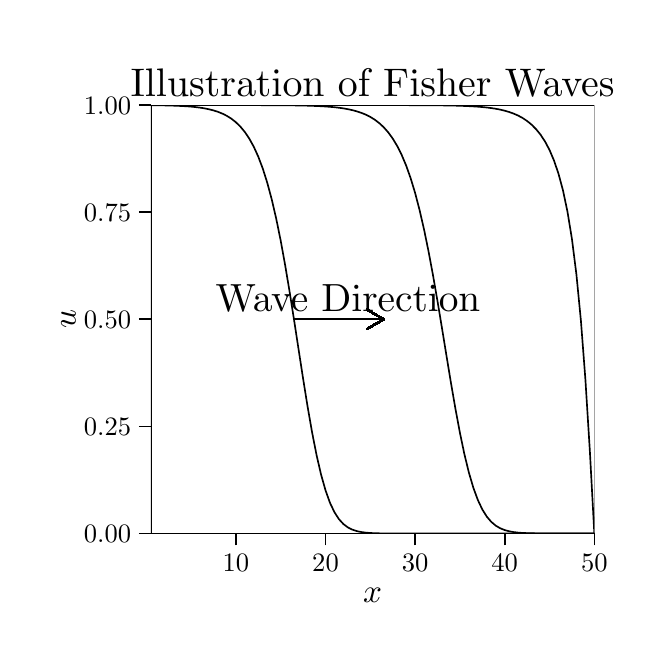
\begin{tikzpicture}[x=1pt,y=1pt]
\definecolor[named]{fillColor}{rgb}{1.00,1.00,1.00}
\path[use as bounding box,fill=fillColor,fill opacity=0.00] (0,0) rectangle (216.81,216.81);
\begin{scope}
\path[clip] (  0.00,  0.00) rectangle (216.81,216.81);
\definecolor[named]{drawColor}{rgb}{1.00,1.00,1.00}
\definecolor[named]{fillColor}{rgb}{1.00,1.00,1.00}

\path[draw=drawColor,line width= 0.6pt,line join=round,line cap=round,fill=fillColor] ( -0.00,  0.00) rectangle (216.81,216.81);
\end{scope}
\begin{scope}
\path[clip] ( 44.49, 34.03) rectangle (204.76,188.82);
\definecolor[named]{fillColor}{rgb}{1.00,1.00,1.00}

\path[fill=fillColor] ( 44.49, 34.03) rectangle (204.76,188.82);
\definecolor[named]{drawColor}{rgb}{0.00,0.00,0.00}

\path[draw=drawColor,line width= 0.6pt,line join=round] ( 44.49,188.80) --
	( 46.10,188.78) --
	( 47.72,188.75) --
	( 49.34,188.72) --
	( 50.96,188.68) --
	( 52.58,188.63) --
	( 54.20,188.57) --
	( 55.82,188.49) --
	( 57.44,188.40) --
	( 59.06,188.27) --
	( 60.68,188.11) --
	( 62.29,187.91) --
	( 63.91,187.65) --
	( 65.53,187.32) --
	( 67.15,186.91) --
	( 68.77,186.39) --
	( 70.39,185.74) --
	( 72.01,184.92) --
	( 73.63,183.90) --
	( 75.25,182.62) --
	( 76.87,181.04) --
	( 78.48,179.09) --
	( 80.10,176.68) --
	( 81.72,173.74) --
	( 83.34,170.17) --
	( 84.96,165.87) --
	( 86.58,160.75) --
	( 88.20,154.72) --
	( 89.82,147.74) --
	( 91.44,139.79) --
	( 93.05,130.91) --
	( 94.67,121.24) --
	( 96.29,110.98) --
	( 97.91,100.43) --
	( 99.53, 89.93) --
	(101.15, 79.86) --
	(102.77, 70.58) --
	(104.39, 62.35) --
	(106.01, 55.34) --
	(107.63, 49.61) --
	(109.24, 45.11) --
	(110.86, 41.70) --
	(112.48, 39.20) --
	(114.10, 37.43) --
	(115.72, 36.22) --
	(117.34, 35.41) --
	(118.96, 34.88) --
	(120.58, 34.55) --
	(122.20, 34.34) --
	(123.82, 34.21) --
	(125.43, 34.14) --
	(127.05, 34.09) --
	(128.67, 34.07) --
	(130.29, 34.05) --
	(131.91, 34.04) --
	(133.53, 34.04) --
	(135.15, 34.04) --
	(136.77, 34.04) --
	(138.39, 34.04) --
	(140.01, 34.03) --
	(141.62, 34.03) --
	(143.24, 34.03) --
	(144.86, 34.03) --
	(146.48, 34.03) --
	(148.10, 34.03) --
	(149.72, 34.03) --
	(151.34, 34.03) --
	(152.96, 34.03) --
	(154.58, 34.03) --
	(156.20, 34.03) --
	(157.81, 34.03) --
	(159.43, 34.03) --
	(161.05, 34.03) --
	(162.67, 34.03) --
	(164.29, 34.03) --
	(165.91, 34.03) --
	(167.53, 34.03) --
	(169.15, 34.03) --
	(170.77, 34.03) --
	(172.39, 34.03) --
	(174.00, 34.03) --
	(175.62, 34.03) --
	(177.24, 34.03) --
	(178.86, 34.03) --
	(180.48, 34.03) --
	(182.10, 34.03) --
	(183.72, 34.03) --
	(185.34, 34.03) --
	(186.96, 34.03) --
	(188.58, 34.03) --
	(190.19, 34.03) --
	(191.81, 34.03) --
	(193.43, 34.03) --
	(195.05, 34.03) --
	(196.67, 34.03) --
	(198.29, 34.03) --
	(199.91, 34.03) --
	(201.53, 34.03) --
	(203.15, 34.03) --
	(204.76, 34.03);

\path[draw=drawColor,line width= 0.6pt,line join=round] ( 44.49,188.82) --
	( 46.10,188.82) --
	( 47.72,188.82) --
	( 49.34,188.82) --
	( 50.96,188.82) --
	( 52.58,188.82) --
	( 54.20,188.82) --
	( 55.82,188.82) --
	( 57.44,188.82) --
	( 59.06,188.82) --
	( 60.68,188.82) --
	( 62.29,188.82) --
	( 63.91,188.82) --
	( 65.53,188.82) --
	( 67.15,188.82) --
	( 68.77,188.82) --
	( 70.39,188.82) --
	( 72.01,188.82) --
	( 73.63,188.82) --
	( 75.25,188.82) --
	( 76.87,188.82) --
	( 78.48,188.82) --
	( 80.10,188.81) --
	( 81.72,188.81) --
	( 83.34,188.81) --
	( 84.96,188.80) --
	( 86.58,188.80) --
	( 88.20,188.79) --
	( 89.82,188.78) --
	( 91.44,188.77) --
	( 93.05,188.75) --
	( 94.67,188.74) --
	( 96.29,188.72) --
	( 97.91,188.69) --
	( 99.53,188.66) --
	(101.15,188.62) --
	(102.77,188.56) --
	(104.39,188.50) --
	(106.01,188.42) --
	(107.63,188.33) --
	(109.24,188.20) --
	(110.86,188.06) --
	(112.48,187.87) --
	(114.10,187.64) --
	(115.72,187.35) --
	(117.34,187.00) --
	(118.96,186.57) --
	(120.58,186.03) --
	(122.20,185.37) --
	(123.82,184.55) --
	(125.43,183.55) --
	(127.05,182.31) --
	(128.67,180.81) --
	(130.29,178.97) --
	(131.91,176.74) --
	(133.53,174.05) --
	(135.15,170.82) --
	(136.77,166.96) --
	(138.39,162.39) --
	(140.01,157.05) --
	(141.62,150.86) --
	(143.24,143.82) --
	(144.86,135.92) --
	(146.48,127.25) --
	(148.10,117.93) --
	(149.72,108.16) --
	(151.34, 98.22) --
	(152.96, 88.40) --
	(154.58, 79.03) --
	(156.20, 70.38) --
	(157.81, 62.67) --
	(159.43, 56.04) --
	(161.05, 50.54) --
	(162.67, 46.13) --
	(164.29, 42.70) --
	(165.91, 40.12) --
	(167.53, 38.22) --
	(169.15, 36.86) --
	(170.77, 35.91) --
	(172.39, 35.26) --
	(174.00, 34.83) --
	(175.62, 34.54) --
	(177.24, 34.35) --
	(178.86, 34.23) --
	(180.48, 34.16) --
	(182.10, 34.11) --
	(183.72, 34.08) --
	(185.34, 34.06) --
	(186.96, 34.05) --
	(188.58, 34.04) --
	(190.19, 34.04) --
	(191.81, 34.04) --
	(193.43, 34.04) --
	(195.05, 34.04) --
	(196.67, 34.04) --
	(198.29, 34.03) --
	(199.91, 34.03) --
	(201.53, 34.03) --
	(203.15, 34.03) --
	(204.76, 34.03);

\path[draw=drawColor,line width= 0.6pt,line join=round] ( 44.49,188.82) --
	( 46.10,188.82) --
	( 47.72,188.82) --
	( 49.34,188.82) --
	( 50.96,188.82) --
	( 52.58,188.82) --
	( 54.20,188.82) --
	( 55.82,188.82) --
	( 57.44,188.82) --
	( 59.06,188.82) --
	( 60.68,188.82) --
	( 62.29,188.82) --
	( 63.91,188.82) --
	( 65.53,188.82) --
	( 67.15,188.82) --
	( 68.77,188.82) --
	( 70.39,188.82) --
	( 72.01,188.82) --
	( 73.63,188.82) --
	( 75.25,188.82) --
	( 76.87,188.82) --
	( 78.48,188.82) --
	( 80.10,188.82) --
	( 81.72,188.82) --
	( 83.34,188.82) --
	( 84.96,188.82) --
	( 86.58,188.82) --
	( 88.20,188.82) --
	( 89.82,188.82) --
	( 91.44,188.82) --
	( 93.05,188.82) --
	( 94.67,188.82) --
	( 96.29,188.82) --
	( 97.91,188.82) --
	( 99.53,188.82) --
	(101.15,188.82) --
	(102.77,188.82) --
	(104.39,188.82) --
	(106.01,188.82) --
	(107.63,188.82) --
	(109.24,188.82) --
	(110.86,188.82) --
	(112.48,188.82) --
	(114.10,188.82) --
	(115.72,188.82) --
	(117.34,188.82) --
	(118.96,188.82) --
	(120.58,188.82) --
	(122.20,188.82) --
	(123.82,188.82) --
	(125.43,188.82) --
	(127.05,188.82) --
	(128.67,188.82) --
	(130.29,188.82) --
	(131.91,188.81) --
	(133.53,188.81) --
	(135.15,188.81) --
	(136.77,188.81) --
	(138.39,188.80) --
	(140.01,188.80) --
	(141.62,188.79) --
	(143.24,188.78) --
	(144.86,188.77) --
	(146.48,188.76) --
	(148.10,188.74) --
	(149.72,188.72) --
	(151.34,188.70) --
	(152.96,188.67) --
	(154.58,188.63) --
	(156.20,188.58) --
	(157.81,188.52) --
	(159.43,188.45) --
	(161.05,188.36) --
	(162.67,188.26) --
	(164.29,188.12) --
	(165.91,187.96) --
	(167.53,187.75) --
	(169.15,187.50) --
	(170.77,187.19) --
	(172.39,186.80) --
	(174.00,186.33) --
	(175.62,185.75) --
	(177.24,185.04) --
	(178.86,184.16) --
	(180.48,183.08) --
	(182.10,181.75) --
	(183.72,180.12) --
	(185.34,178.12) --
	(186.96,175.65) --
	(188.58,172.59) --
	(190.19,168.79) --
	(191.81,164.03) --
	(193.43,158.02) --
	(195.05,150.34) --
	(196.67,140.44) --
	(198.29,127.59) --
	(199.91,110.94) --
	(201.53, 89.72) --
	(203.15, 63.70) --
	(204.76, 34.03);
\definecolor[named]{fillColor}{rgb}{0.00,0.00,0.00}

\path[draw=drawColor,line width= 0.6pt,line join=round,fill=fillColor] ( 96.29,111.43) -- (128.67,111.43);

\path[draw=drawColor,line width= 0.6pt,line join=round] (122.51,107.87) --
	(128.67,111.43) --
	(122.51,114.99);

\path[draw=drawColor,line width= 0.6pt,line join=round,fill=fillColor] ( 96.29,111.43) -- (128.67,111.43);

\path[draw=drawColor,line width= 0.6pt,line join=round] (122.51,107.87) --
	(128.67,111.43) --
	(122.51,114.99);

\path[draw=drawColor,line width= 0.6pt,line join=round,fill=fillColor] ( 96.29,111.43) -- (128.67,111.43);

\path[draw=drawColor,line width= 0.6pt,line join=round] (122.51,107.87) --
	(128.67,111.43) --
	(122.51,114.99);

\path[draw=drawColor,line width= 0.6pt,line join=round,fill=fillColor] ( 96.29,111.43) -- (128.67,111.43);

\path[draw=drawColor,line width= 0.6pt,line join=round] (122.51,107.87) --
	(128.67,111.43) --
	(122.51,114.99);

\path[draw=drawColor,line width= 0.6pt,line join=round,fill=fillColor] ( 96.29,111.43) -- (128.67,111.43);

\path[draw=drawColor,line width= 0.6pt,line join=round] (122.51,107.87) --
	(128.67,111.43) --
	(122.51,114.99);

\path[draw=drawColor,line width= 0.6pt,line join=round,fill=fillColor] ( 96.29,111.43) -- (128.67,111.43);

\path[draw=drawColor,line width= 0.6pt,line join=round] (122.51,107.87) --
	(128.67,111.43) --
	(122.51,114.99);

\path[draw=drawColor,line width= 0.6pt,line join=round,fill=fillColor] ( 96.29,111.43) -- (128.67,111.43);

\path[draw=drawColor,line width= 0.6pt,line join=round] (122.51,107.87) --
	(128.67,111.43) --
	(122.51,114.99);

\path[draw=drawColor,line width= 0.6pt,line join=round,fill=fillColor] ( 96.29,111.43) -- (128.67,111.43);

\path[draw=drawColor,line width= 0.6pt,line join=round] (122.51,107.87) --
	(128.67,111.43) --
	(122.51,114.99);

\path[draw=drawColor,line width= 0.6pt,line join=round,fill=fillColor] ( 96.29,111.43) -- (128.67,111.43);

\path[draw=drawColor,line width= 0.6pt,line join=round] (122.51,107.87) --
	(128.67,111.43) --
	(122.51,114.99);

\path[draw=drawColor,line width= 0.6pt,line join=round,fill=fillColor] ( 96.29,111.43) -- (128.67,111.43);

\path[draw=drawColor,line width= 0.6pt,line join=round] (122.51,107.87) --
	(128.67,111.43) --
	(122.51,114.99);

\path[draw=drawColor,line width= 0.6pt,line join=round,fill=fillColor] ( 96.29,111.43) -- (128.67,111.43);

\path[draw=drawColor,line width= 0.6pt,line join=round] (122.51,107.87) --
	(128.67,111.43) --
	(122.51,114.99);

\path[draw=drawColor,line width= 0.6pt,line join=round,fill=fillColor] ( 96.29,111.43) -- (128.67,111.43);

\path[draw=drawColor,line width= 0.6pt,line join=round] (122.51,107.87) --
	(128.67,111.43) --
	(122.51,114.99);

\path[draw=drawColor,line width= 0.6pt,line join=round,fill=fillColor] ( 96.29,111.43) -- (128.67,111.43);

\path[draw=drawColor,line width= 0.6pt,line join=round] (122.51,107.87) --
	(128.67,111.43) --
	(122.51,114.99);

\path[draw=drawColor,line width= 0.6pt,line join=round,fill=fillColor] ( 96.29,111.43) -- (128.67,111.43);

\path[draw=drawColor,line width= 0.6pt,line join=round] (122.51,107.87) --
	(128.67,111.43) --
	(122.51,114.99);

\path[draw=drawColor,line width= 0.6pt,line join=round,fill=fillColor] ( 96.29,111.43) -- (128.67,111.43);

\path[draw=drawColor,line width= 0.6pt,line join=round] (122.51,107.87) --
	(128.67,111.43) --
	(122.51,114.99);

\path[draw=drawColor,line width= 0.6pt,line join=round,fill=fillColor] ( 96.29,111.43) -- (128.67,111.43);

\path[draw=drawColor,line width= 0.6pt,line join=round] (122.51,107.87) --
	(128.67,111.43) --
	(122.51,114.99);

\path[draw=drawColor,line width= 0.6pt,line join=round,fill=fillColor] ( 96.29,111.43) -- (128.67,111.43);

\path[draw=drawColor,line width= 0.6pt,line join=round] (122.51,107.87) --
	(128.67,111.43) --
	(122.51,114.99);

\path[draw=drawColor,line width= 0.6pt,line join=round,fill=fillColor] ( 96.29,111.43) -- (128.67,111.43);

\path[draw=drawColor,line width= 0.6pt,line join=round] (122.51,107.87) --
	(128.67,111.43) --
	(122.51,114.99);

\path[draw=drawColor,line width= 0.6pt,line join=round,fill=fillColor] ( 96.29,111.43) -- (128.67,111.43);

\path[draw=drawColor,line width= 0.6pt,line join=round] (122.51,107.87) --
	(128.67,111.43) --
	(122.51,114.99);

\path[draw=drawColor,line width= 0.6pt,line join=round,fill=fillColor] ( 96.29,111.43) -- (128.67,111.43);

\path[draw=drawColor,line width= 0.6pt,line join=round] (122.51,107.87) --
	(128.67,111.43) --
	(122.51,114.99);

\path[draw=drawColor,line width= 0.6pt,line join=round,fill=fillColor] ( 96.29,111.43) -- (128.67,111.43);

\path[draw=drawColor,line width= 0.6pt,line join=round] (122.51,107.87) --
	(128.67,111.43) --
	(122.51,114.99);

\path[draw=drawColor,line width= 0.6pt,line join=round,fill=fillColor] ( 96.29,111.43) -- (128.67,111.43);

\path[draw=drawColor,line width= 0.6pt,line join=round] (122.51,107.87) --
	(128.67,111.43) --
	(122.51,114.99);

\path[draw=drawColor,line width= 0.6pt,line join=round,fill=fillColor] ( 96.29,111.43) -- (128.67,111.43);

\path[draw=drawColor,line width= 0.6pt,line join=round] (122.51,107.87) --
	(128.67,111.43) --
	(122.51,114.99);

\path[draw=drawColor,line width= 0.6pt,line join=round,fill=fillColor] ( 96.29,111.43) -- (128.67,111.43);

\path[draw=drawColor,line width= 0.6pt,line join=round] (122.51,107.87) --
	(128.67,111.43) --
	(122.51,114.99);

\path[draw=drawColor,line width= 0.6pt,line join=round,fill=fillColor] ( 96.29,111.43) -- (128.67,111.43);

\path[draw=drawColor,line width= 0.6pt,line join=round] (122.51,107.87) --
	(128.67,111.43) --
	(122.51,114.99);

\path[draw=drawColor,line width= 0.6pt,line join=round,fill=fillColor] ( 96.29,111.43) -- (128.67,111.43);

\path[draw=drawColor,line width= 0.6pt,line join=round] (122.51,107.87) --
	(128.67,111.43) --
	(122.51,114.99);

\path[draw=drawColor,line width= 0.6pt,line join=round,fill=fillColor] ( 96.29,111.43) -- (128.67,111.43);

\path[draw=drawColor,line width= 0.6pt,line join=round] (122.51,107.87) --
	(128.67,111.43) --
	(122.51,114.99);

\path[draw=drawColor,line width= 0.6pt,line join=round,fill=fillColor] ( 96.29,111.43) -- (128.67,111.43);

\path[draw=drawColor,line width= 0.6pt,line join=round] (122.51,107.87) --
	(128.67,111.43) --
	(122.51,114.99);

\path[draw=drawColor,line width= 0.6pt,line join=round,fill=fillColor] ( 96.29,111.43) -- (128.67,111.43);

\path[draw=drawColor,line width= 0.6pt,line join=round] (122.51,107.87) --
	(128.67,111.43) --
	(122.51,114.99);

\path[draw=drawColor,line width= 0.6pt,line join=round,fill=fillColor] ( 96.29,111.43) -- (128.67,111.43);

\path[draw=drawColor,line width= 0.6pt,line join=round] (122.51,107.87) --
	(128.67,111.43) --
	(122.51,114.99);

\path[draw=drawColor,line width= 0.6pt,line join=round,fill=fillColor] ( 96.29,111.43) -- (128.67,111.43);

\path[draw=drawColor,line width= 0.6pt,line join=round] (122.51,107.87) --
	(128.67,111.43) --
	(122.51,114.99);

\path[draw=drawColor,line width= 0.6pt,line join=round,fill=fillColor] ( 96.29,111.43) -- (128.67,111.43);

\path[draw=drawColor,line width= 0.6pt,line join=round] (122.51,107.87) --
	(128.67,111.43) --
	(122.51,114.99);

\path[draw=drawColor,line width= 0.6pt,line join=round,fill=fillColor] ( 96.29,111.43) -- (128.67,111.43);

\path[draw=drawColor,line width= 0.6pt,line join=round] (122.51,107.87) --
	(128.67,111.43) --
	(122.51,114.99);

\path[draw=drawColor,line width= 0.6pt,line join=round,fill=fillColor] ( 96.29,111.43) -- (128.67,111.43);

\path[draw=drawColor,line width= 0.6pt,line join=round] (122.51,107.87) --
	(128.67,111.43) --
	(122.51,114.99);

\path[draw=drawColor,line width= 0.6pt,line join=round,fill=fillColor] ( 96.29,111.43) -- (128.67,111.43);

\path[draw=drawColor,line width= 0.6pt,line join=round] (122.51,107.87) --
	(128.67,111.43) --
	(122.51,114.99);

\path[draw=drawColor,line width= 0.6pt,line join=round,fill=fillColor] ( 96.29,111.43) -- (128.67,111.43);

\path[draw=drawColor,line width= 0.6pt,line join=round] (122.51,107.87) --
	(128.67,111.43) --
	(122.51,114.99);

\path[draw=drawColor,line width= 0.6pt,line join=round,fill=fillColor] ( 96.29,111.43) -- (128.67,111.43);

\path[draw=drawColor,line width= 0.6pt,line join=round] (122.51,107.87) --
	(128.67,111.43) --
	(122.51,114.99);

\path[draw=drawColor,line width= 0.6pt,line join=round,fill=fillColor] ( 96.29,111.43) -- (128.67,111.43);

\path[draw=drawColor,line width= 0.6pt,line join=round] (122.51,107.87) --
	(128.67,111.43) --
	(122.51,114.99);

\path[draw=drawColor,line width= 0.6pt,line join=round,fill=fillColor] ( 96.29,111.43) -- (128.67,111.43);

\path[draw=drawColor,line width= 0.6pt,line join=round] (122.51,107.87) --
	(128.67,111.43) --
	(122.51,114.99);

\path[draw=drawColor,line width= 0.6pt,line join=round,fill=fillColor] ( 96.29,111.43) -- (128.67,111.43);

\path[draw=drawColor,line width= 0.6pt,line join=round] (122.51,107.87) --
	(128.67,111.43) --
	(122.51,114.99);

\path[draw=drawColor,line width= 0.6pt,line join=round,fill=fillColor] ( 96.29,111.43) -- (128.67,111.43);

\path[draw=drawColor,line width= 0.6pt,line join=round] (122.51,107.87) --
	(128.67,111.43) --
	(122.51,114.99);

\path[draw=drawColor,line width= 0.6pt,line join=round,fill=fillColor] ( 96.29,111.43) -- (128.67,111.43);

\path[draw=drawColor,line width= 0.6pt,line join=round] (122.51,107.87) --
	(128.67,111.43) --
	(122.51,114.99);

\path[draw=drawColor,line width= 0.6pt,line join=round,fill=fillColor] ( 96.29,111.43) -- (128.67,111.43);

\path[draw=drawColor,line width= 0.6pt,line join=round] (122.51,107.87) --
	(128.67,111.43) --
	(122.51,114.99);

\path[draw=drawColor,line width= 0.6pt,line join=round,fill=fillColor] ( 96.29,111.43) -- (128.67,111.43);

\path[draw=drawColor,line width= 0.6pt,line join=round] (122.51,107.87) --
	(128.67,111.43) --
	(122.51,114.99);

\path[draw=drawColor,line width= 0.6pt,line join=round,fill=fillColor] ( 96.29,111.43) -- (128.67,111.43);

\path[draw=drawColor,line width= 0.6pt,line join=round] (122.51,107.87) --
	(128.67,111.43) --
	(122.51,114.99);

\path[draw=drawColor,line width= 0.6pt,line join=round,fill=fillColor] ( 96.29,111.43) -- (128.67,111.43);

\path[draw=drawColor,line width= 0.6pt,line join=round] (122.51,107.87) --
	(128.67,111.43) --
	(122.51,114.99);

\path[draw=drawColor,line width= 0.6pt,line join=round,fill=fillColor] ( 96.29,111.43) -- (128.67,111.43);

\path[draw=drawColor,line width= 0.6pt,line join=round] (122.51,107.87) --
	(128.67,111.43) --
	(122.51,114.99);

\path[draw=drawColor,line width= 0.6pt,line join=round,fill=fillColor] ( 96.29,111.43) -- (128.67,111.43);

\path[draw=drawColor,line width= 0.6pt,line join=round] (122.51,107.87) --
	(128.67,111.43) --
	(122.51,114.99);

\path[draw=drawColor,line width= 0.6pt,line join=round,fill=fillColor] ( 96.29,111.43) -- (128.67,111.43);

\path[draw=drawColor,line width= 0.6pt,line join=round] (122.51,107.87) --
	(128.67,111.43) --
	(122.51,114.99);

\path[draw=drawColor,line width= 0.6pt,line join=round,fill=fillColor] ( 96.29,111.43) -- (128.67,111.43);

\path[draw=drawColor,line width= 0.6pt,line join=round] (122.51,107.87) --
	(128.67,111.43) --
	(122.51,114.99);

\path[draw=drawColor,line width= 0.6pt,line join=round,fill=fillColor] ( 96.29,111.43) -- (128.67,111.43);

\path[draw=drawColor,line width= 0.6pt,line join=round] (122.51,107.87) --
	(128.67,111.43) --
	(122.51,114.99);

\path[draw=drawColor,line width= 0.6pt,line join=round,fill=fillColor] ( 96.29,111.43) -- (128.67,111.43);

\path[draw=drawColor,line width= 0.6pt,line join=round] (122.51,107.87) --
	(128.67,111.43) --
	(122.51,114.99);

\path[draw=drawColor,line width= 0.6pt,line join=round,fill=fillColor] ( 96.29,111.43) -- (128.67,111.43);

\path[draw=drawColor,line width= 0.6pt,line join=round] (122.51,107.87) --
	(128.67,111.43) --
	(122.51,114.99);

\path[draw=drawColor,line width= 0.6pt,line join=round,fill=fillColor] ( 96.29,111.43) -- (128.67,111.43);

\path[draw=drawColor,line width= 0.6pt,line join=round] (122.51,107.87) --
	(128.67,111.43) --
	(122.51,114.99);

\path[draw=drawColor,line width= 0.6pt,line join=round,fill=fillColor] ( 96.29,111.43) -- (128.67,111.43);

\path[draw=drawColor,line width= 0.6pt,line join=round] (122.51,107.87) --
	(128.67,111.43) --
	(122.51,114.99);

\path[draw=drawColor,line width= 0.6pt,line join=round,fill=fillColor] ( 96.29,111.43) -- (128.67,111.43);

\path[draw=drawColor,line width= 0.6pt,line join=round] (122.51,107.87) --
	(128.67,111.43) --
	(122.51,114.99);

\path[draw=drawColor,line width= 0.6pt,line join=round,fill=fillColor] ( 96.29,111.43) -- (128.67,111.43);

\path[draw=drawColor,line width= 0.6pt,line join=round] (122.51,107.87) --
	(128.67,111.43) --
	(122.51,114.99);

\path[draw=drawColor,line width= 0.6pt,line join=round,fill=fillColor] ( 96.29,111.43) -- (128.67,111.43);

\path[draw=drawColor,line width= 0.6pt,line join=round] (122.51,107.87) --
	(128.67,111.43) --
	(122.51,114.99);

\path[draw=drawColor,line width= 0.6pt,line join=round,fill=fillColor] ( 96.29,111.43) -- (128.67,111.43);

\path[draw=drawColor,line width= 0.6pt,line join=round] (122.51,107.87) --
	(128.67,111.43) --
	(122.51,114.99);

\path[draw=drawColor,line width= 0.6pt,line join=round,fill=fillColor] ( 96.29,111.43) -- (128.67,111.43);

\path[draw=drawColor,line width= 0.6pt,line join=round] (122.51,107.87) --
	(128.67,111.43) --
	(122.51,114.99);

\path[draw=drawColor,line width= 0.6pt,line join=round,fill=fillColor] ( 96.29,111.43) -- (128.67,111.43);

\path[draw=drawColor,line width= 0.6pt,line join=round] (122.51,107.87) --
	(128.67,111.43) --
	(122.51,114.99);

\path[draw=drawColor,line width= 0.6pt,line join=round,fill=fillColor] ( 96.29,111.43) -- (128.67,111.43);

\path[draw=drawColor,line width= 0.6pt,line join=round] (122.51,107.87) --
	(128.67,111.43) --
	(122.51,114.99);

\path[draw=drawColor,line width= 0.6pt,line join=round,fill=fillColor] ( 96.29,111.43) -- (128.67,111.43);

\path[draw=drawColor,line width= 0.6pt,line join=round] (122.51,107.87) --
	(128.67,111.43) --
	(122.51,114.99);

\path[draw=drawColor,line width= 0.6pt,line join=round,fill=fillColor] ( 96.29,111.43) -- (128.67,111.43);

\path[draw=drawColor,line width= 0.6pt,line join=round] (122.51,107.87) --
	(128.67,111.43) --
	(122.51,114.99);

\path[draw=drawColor,line width= 0.6pt,line join=round,fill=fillColor] ( 96.29,111.43) -- (128.67,111.43);

\path[draw=drawColor,line width= 0.6pt,line join=round] (122.51,107.87) --
	(128.67,111.43) --
	(122.51,114.99);

\path[draw=drawColor,line width= 0.6pt,line join=round,fill=fillColor] ( 96.29,111.43) -- (128.67,111.43);

\path[draw=drawColor,line width= 0.6pt,line join=round] (122.51,107.87) --
	(128.67,111.43) --
	(122.51,114.99);

\path[draw=drawColor,line width= 0.6pt,line join=round,fill=fillColor] ( 96.29,111.43) -- (128.67,111.43);

\path[draw=drawColor,line width= 0.6pt,line join=round] (122.51,107.87) --
	(128.67,111.43) --
	(122.51,114.99);

\path[draw=drawColor,line width= 0.6pt,line join=round,fill=fillColor] ( 96.29,111.43) -- (128.67,111.43);

\path[draw=drawColor,line width= 0.6pt,line join=round] (122.51,107.87) --
	(128.67,111.43) --
	(122.51,114.99);

\path[draw=drawColor,line width= 0.6pt,line join=round,fill=fillColor] ( 96.29,111.43) -- (128.67,111.43);

\path[draw=drawColor,line width= 0.6pt,line join=round] (122.51,107.87) --
	(128.67,111.43) --
	(122.51,114.99);

\path[draw=drawColor,line width= 0.6pt,line join=round,fill=fillColor] ( 96.29,111.43) -- (128.67,111.43);

\path[draw=drawColor,line width= 0.6pt,line join=round] (122.51,107.87) --
	(128.67,111.43) --
	(122.51,114.99);

\path[draw=drawColor,line width= 0.6pt,line join=round,fill=fillColor] ( 96.29,111.43) -- (128.67,111.43);

\path[draw=drawColor,line width= 0.6pt,line join=round] (122.51,107.87) --
	(128.67,111.43) --
	(122.51,114.99);

\path[draw=drawColor,line width= 0.6pt,line join=round,fill=fillColor] ( 96.29,111.43) -- (128.67,111.43);

\path[draw=drawColor,line width= 0.6pt,line join=round] (122.51,107.87) --
	(128.67,111.43) --
	(122.51,114.99);

\path[draw=drawColor,line width= 0.6pt,line join=round,fill=fillColor] ( 96.29,111.43) -- (128.67,111.43);

\path[draw=drawColor,line width= 0.6pt,line join=round] (122.51,107.87) --
	(128.67,111.43) --
	(122.51,114.99);

\path[draw=drawColor,line width= 0.6pt,line join=round,fill=fillColor] ( 96.29,111.43) -- (128.67,111.43);

\path[draw=drawColor,line width= 0.6pt,line join=round] (122.51,107.87) --
	(128.67,111.43) --
	(122.51,114.99);

\path[draw=drawColor,line width= 0.6pt,line join=round,fill=fillColor] ( 96.29,111.43) -- (128.67,111.43);

\path[draw=drawColor,line width= 0.6pt,line join=round] (122.51,107.87) --
	(128.67,111.43) --
	(122.51,114.99);

\path[draw=drawColor,line width= 0.6pt,line join=round,fill=fillColor] ( 96.29,111.43) -- (128.67,111.43);

\path[draw=drawColor,line width= 0.6pt,line join=round] (122.51,107.87) --
	(128.67,111.43) --
	(122.51,114.99);

\path[draw=drawColor,line width= 0.6pt,line join=round,fill=fillColor] ( 96.29,111.43) -- (128.67,111.43);

\path[draw=drawColor,line width= 0.6pt,line join=round] (122.51,107.87) --
	(128.67,111.43) --
	(122.51,114.99);

\path[draw=drawColor,line width= 0.6pt,line join=round,fill=fillColor] ( 96.29,111.43) -- (128.67,111.43);

\path[draw=drawColor,line width= 0.6pt,line join=round] (122.51,107.87) --
	(128.67,111.43) --
	(122.51,114.99);

\path[draw=drawColor,line width= 0.6pt,line join=round,fill=fillColor] ( 96.29,111.43) -- (128.67,111.43);

\path[draw=drawColor,line width= 0.6pt,line join=round] (122.51,107.87) --
	(128.67,111.43) --
	(122.51,114.99);

\path[draw=drawColor,line width= 0.6pt,line join=round,fill=fillColor] ( 96.29,111.43) -- (128.67,111.43);

\path[draw=drawColor,line width= 0.6pt,line join=round] (122.51,107.87) --
	(128.67,111.43) --
	(122.51,114.99);

\path[draw=drawColor,line width= 0.6pt,line join=round,fill=fillColor] ( 96.29,111.43) -- (128.67,111.43);

\path[draw=drawColor,line width= 0.6pt,line join=round] (122.51,107.87) --
	(128.67,111.43) --
	(122.51,114.99);

\path[draw=drawColor,line width= 0.6pt,line join=round,fill=fillColor] ( 96.29,111.43) -- (128.67,111.43);

\path[draw=drawColor,line width= 0.6pt,line join=round] (122.51,107.87) --
	(128.67,111.43) --
	(122.51,114.99);

\path[draw=drawColor,line width= 0.6pt,line join=round,fill=fillColor] ( 96.29,111.43) -- (128.67,111.43);

\path[draw=drawColor,line width= 0.6pt,line join=round] (122.51,107.87) --
	(128.67,111.43) --
	(122.51,114.99);

\path[draw=drawColor,line width= 0.6pt,line join=round,fill=fillColor] ( 96.29,111.43) -- (128.67,111.43);

\path[draw=drawColor,line width= 0.6pt,line join=round] (122.51,107.87) --
	(128.67,111.43) --
	(122.51,114.99);

\path[draw=drawColor,line width= 0.6pt,line join=round,fill=fillColor] ( 96.29,111.43) -- (128.67,111.43);

\path[draw=drawColor,line width= 0.6pt,line join=round] (122.51,107.87) --
	(128.67,111.43) --
	(122.51,114.99);

\path[draw=drawColor,line width= 0.6pt,line join=round,fill=fillColor] ( 96.29,111.43) -- (128.67,111.43);

\path[draw=drawColor,line width= 0.6pt,line join=round] (122.51,107.87) --
	(128.67,111.43) --
	(122.51,114.99);

\path[draw=drawColor,line width= 0.6pt,line join=round,fill=fillColor] ( 96.29,111.43) -- (128.67,111.43);

\path[draw=drawColor,line width= 0.6pt,line join=round] (122.51,107.87) --
	(128.67,111.43) --
	(122.51,114.99);

\path[draw=drawColor,line width= 0.6pt,line join=round,fill=fillColor] ( 96.29,111.43) -- (128.67,111.43);

\path[draw=drawColor,line width= 0.6pt,line join=round] (122.51,107.87) --
	(128.67,111.43) --
	(122.51,114.99);

\path[draw=drawColor,line width= 0.6pt,line join=round,fill=fillColor] ( 96.29,111.43) -- (128.67,111.43);

\path[draw=drawColor,line width= 0.6pt,line join=round] (122.51,107.87) --
	(128.67,111.43) --
	(122.51,114.99);

\path[draw=drawColor,line width= 0.6pt,line join=round,fill=fillColor] ( 96.29,111.43) -- (128.67,111.43);

\path[draw=drawColor,line width= 0.6pt,line join=round] (122.51,107.87) --
	(128.67,111.43) --
	(122.51,114.99);

\path[draw=drawColor,line width= 0.6pt,line join=round,fill=fillColor] ( 96.29,111.43) -- (128.67,111.43);

\path[draw=drawColor,line width= 0.6pt,line join=round] (122.51,107.87) --
	(128.67,111.43) --
	(122.51,114.99);

\path[draw=drawColor,line width= 0.6pt,line join=round,fill=fillColor] ( 96.29,111.43) -- (128.67,111.43);

\path[draw=drawColor,line width= 0.6pt,line join=round] (122.51,107.87) --
	(128.67,111.43) --
	(122.51,114.99);

\path[draw=drawColor,line width= 0.6pt,line join=round,fill=fillColor] ( 96.29,111.43) -- (128.67,111.43);

\path[draw=drawColor,line width= 0.6pt,line join=round] (122.51,107.87) --
	(128.67,111.43) --
	(122.51,114.99);

\path[draw=drawColor,line width= 0.6pt,line join=round,fill=fillColor] ( 96.29,111.43) -- (128.67,111.43);

\path[draw=drawColor,line width= 0.6pt,line join=round] (122.51,107.87) --
	(128.67,111.43) --
	(122.51,114.99);

\path[draw=drawColor,line width= 0.6pt,line join=round,fill=fillColor] ( 96.29,111.43) -- (128.67,111.43);

\path[draw=drawColor,line width= 0.6pt,line join=round] (122.51,107.87) --
	(128.67,111.43) --
	(122.51,114.99);

\path[draw=drawColor,line width= 0.6pt,line join=round,fill=fillColor] ( 96.29,111.43) -- (128.67,111.43);

\path[draw=drawColor,line width= 0.6pt,line join=round] (122.51,107.87) --
	(128.67,111.43) --
	(122.51,114.99);

\path[draw=drawColor,line width= 0.6pt,line join=round,fill=fillColor] ( 96.29,111.43) -- (128.67,111.43);

\path[draw=drawColor,line width= 0.6pt,line join=round] (122.51,107.87) --
	(128.67,111.43) --
	(122.51,114.99);

\path[draw=drawColor,line width= 0.6pt,line join=round,fill=fillColor] ( 96.29,111.43) -- (128.67,111.43);

\path[draw=drawColor,line width= 0.6pt,line join=round] (122.51,107.87) --
	(128.67,111.43) --
	(122.51,114.99);

\path[draw=drawColor,line width= 0.6pt,line join=round,fill=fillColor] ( 96.29,111.43) -- (128.67,111.43);

\path[draw=drawColor,line width= 0.6pt,line join=round] (122.51,107.87) --
	(128.67,111.43) --
	(122.51,114.99);

\path[draw=drawColor,line width= 0.6pt,line join=round,fill=fillColor] ( 96.29,111.43) -- (128.67,111.43);

\path[draw=drawColor,line width= 0.6pt,line join=round] (122.51,107.87) --
	(128.67,111.43) --
	(122.51,114.99);

\path[draw=drawColor,line width= 0.6pt,line join=round,fill=fillColor] ( 96.29,111.43) -- (128.67,111.43);

\path[draw=drawColor,line width= 0.6pt,line join=round] (122.51,107.87) --
	(128.67,111.43) --
	(122.51,114.99);

\path[draw=drawColor,line width= 0.6pt,line join=round,fill=fillColor] ( 96.29,111.43) -- (128.67,111.43);

\path[draw=drawColor,line width= 0.6pt,line join=round] (122.51,107.87) --
	(128.67,111.43) --
	(122.51,114.99);

\path[draw=drawColor,line width= 0.6pt,line join=round,fill=fillColor] ( 96.29,111.43) -- (128.67,111.43);

\path[draw=drawColor,line width= 0.6pt,line join=round] (122.51,107.87) --
	(128.67,111.43) --
	(122.51,114.99);

\path[draw=drawColor,line width= 0.6pt,line join=round,fill=fillColor] ( 96.29,111.43) -- (128.67,111.43);

\path[draw=drawColor,line width= 0.6pt,line join=round] (122.51,107.87) --
	(128.67,111.43) --
	(122.51,114.99);

\path[draw=drawColor,line width= 0.6pt,line join=round,fill=fillColor] ( 96.29,111.43) -- (128.67,111.43);

\path[draw=drawColor,line width= 0.6pt,line join=round] (122.51,107.87) --
	(128.67,111.43) --
	(122.51,114.99);

\path[draw=drawColor,line width= 0.6pt,line join=round,fill=fillColor] ( 96.29,111.43) -- (128.67,111.43);

\path[draw=drawColor,line width= 0.6pt,line join=round] (122.51,107.87) --
	(128.67,111.43) --
	(122.51,114.99);

\path[draw=drawColor,line width= 0.6pt,line join=round,fill=fillColor] ( 96.29,111.43) -- (128.67,111.43);

\path[draw=drawColor,line width= 0.6pt,line join=round] (122.51,107.87) --
	(128.67,111.43) --
	(122.51,114.99);

\path[draw=drawColor,line width= 0.6pt,line join=round,fill=fillColor] ( 96.29,111.43) -- (128.67,111.43);

\path[draw=drawColor,line width= 0.6pt,line join=round] (122.51,107.87) --
	(128.67,111.43) --
	(122.51,114.99);

\path[draw=drawColor,line width= 0.6pt,line join=round,fill=fillColor] ( 96.29,111.43) -- (128.67,111.43);

\path[draw=drawColor,line width= 0.6pt,line join=round] (122.51,107.87) --
	(128.67,111.43) --
	(122.51,114.99);

\path[draw=drawColor,line width= 0.6pt,line join=round,fill=fillColor] ( 96.29,111.43) -- (128.67,111.43);

\path[draw=drawColor,line width= 0.6pt,line join=round] (122.51,107.87) --
	(128.67,111.43) --
	(122.51,114.99);

\path[draw=drawColor,line width= 0.6pt,line join=round,fill=fillColor] ( 96.29,111.43) -- (128.67,111.43);

\path[draw=drawColor,line width= 0.6pt,line join=round] (122.51,107.87) --
	(128.67,111.43) --
	(122.51,114.99);

\path[draw=drawColor,line width= 0.6pt,line join=round,fill=fillColor] ( 96.29,111.43) -- (128.67,111.43);

\path[draw=drawColor,line width= 0.6pt,line join=round] (122.51,107.87) --
	(128.67,111.43) --
	(122.51,114.99);

\path[draw=drawColor,line width= 0.6pt,line join=round,fill=fillColor] ( 96.29,111.43) -- (128.67,111.43);

\path[draw=drawColor,line width= 0.6pt,line join=round] (122.51,107.87) --
	(128.67,111.43) --
	(122.51,114.99);

\path[draw=drawColor,line width= 0.6pt,line join=round,fill=fillColor] ( 96.29,111.43) -- (128.67,111.43);

\path[draw=drawColor,line width= 0.6pt,line join=round] (122.51,107.87) --
	(128.67,111.43) --
	(122.51,114.99);

\path[draw=drawColor,line width= 0.6pt,line join=round,fill=fillColor] ( 96.29,111.43) -- (128.67,111.43);

\path[draw=drawColor,line width= 0.6pt,line join=round] (122.51,107.87) --
	(128.67,111.43) --
	(122.51,114.99);

\path[draw=drawColor,line width= 0.6pt,line join=round,fill=fillColor] ( 96.29,111.43) -- (128.67,111.43);

\path[draw=drawColor,line width= 0.6pt,line join=round] (122.51,107.87) --
	(128.67,111.43) --
	(122.51,114.99);

\path[draw=drawColor,line width= 0.6pt,line join=round,fill=fillColor] ( 96.29,111.43) -- (128.67,111.43);

\path[draw=drawColor,line width= 0.6pt,line join=round] (122.51,107.87) --
	(128.67,111.43) --
	(122.51,114.99);

\path[draw=drawColor,line width= 0.6pt,line join=round,fill=fillColor] ( 96.29,111.43) -- (128.67,111.43);

\path[draw=drawColor,line width= 0.6pt,line join=round] (122.51,107.87) --
	(128.67,111.43) --
	(122.51,114.99);

\path[draw=drawColor,line width= 0.6pt,line join=round,fill=fillColor] ( 96.29,111.43) -- (128.67,111.43);

\path[draw=drawColor,line width= 0.6pt,line join=round] (122.51,107.87) --
	(128.67,111.43) --
	(122.51,114.99);

\path[draw=drawColor,line width= 0.6pt,line join=round,fill=fillColor] ( 96.29,111.43) -- (128.67,111.43);

\path[draw=drawColor,line width= 0.6pt,line join=round] (122.51,107.87) --
	(128.67,111.43) --
	(122.51,114.99);

\path[draw=drawColor,line width= 0.6pt,line join=round,fill=fillColor] ( 96.29,111.43) -- (128.67,111.43);

\path[draw=drawColor,line width= 0.6pt,line join=round] (122.51,107.87) --
	(128.67,111.43) --
	(122.51,114.99);

\path[draw=drawColor,line width= 0.6pt,line join=round,fill=fillColor] ( 96.29,111.43) -- (128.67,111.43);

\path[draw=drawColor,line width= 0.6pt,line join=round] (122.51,107.87) --
	(128.67,111.43) --
	(122.51,114.99);

\path[draw=drawColor,line width= 0.6pt,line join=round,fill=fillColor] ( 96.29,111.43) -- (128.67,111.43);

\path[draw=drawColor,line width= 0.6pt,line join=round] (122.51,107.87) --
	(128.67,111.43) --
	(122.51,114.99);

\path[draw=drawColor,line width= 0.6pt,line join=round,fill=fillColor] ( 96.29,111.43) -- (128.67,111.43);

\path[draw=drawColor,line width= 0.6pt,line join=round] (122.51,107.87) --
	(128.67,111.43) --
	(122.51,114.99);

\path[draw=drawColor,line width= 0.6pt,line join=round,fill=fillColor] ( 96.29,111.43) -- (128.67,111.43);

\path[draw=drawColor,line width= 0.6pt,line join=round] (122.51,107.87) --
	(128.67,111.43) --
	(122.51,114.99);

\path[draw=drawColor,line width= 0.6pt,line join=round,fill=fillColor] ( 96.29,111.43) -- (128.67,111.43);

\path[draw=drawColor,line width= 0.6pt,line join=round] (122.51,107.87) --
	(128.67,111.43) --
	(122.51,114.99);

\path[draw=drawColor,line width= 0.6pt,line join=round,fill=fillColor] ( 96.29,111.43) -- (128.67,111.43);

\path[draw=drawColor,line width= 0.6pt,line join=round] (122.51,107.87) --
	(128.67,111.43) --
	(122.51,114.99);

\path[draw=drawColor,line width= 0.6pt,line join=round,fill=fillColor] ( 96.29,111.43) -- (128.67,111.43);

\path[draw=drawColor,line width= 0.6pt,line join=round] (122.51,107.87) --
	(128.67,111.43) --
	(122.51,114.99);

\path[draw=drawColor,line width= 0.6pt,line join=round,fill=fillColor] ( 96.29,111.43) -- (128.67,111.43);

\path[draw=drawColor,line width= 0.6pt,line join=round] (122.51,107.87) --
	(128.67,111.43) --
	(122.51,114.99);

\path[draw=drawColor,line width= 0.6pt,line join=round,fill=fillColor] ( 96.29,111.43) -- (128.67,111.43);

\path[draw=drawColor,line width= 0.6pt,line join=round] (122.51,107.87) --
	(128.67,111.43) --
	(122.51,114.99);

\path[draw=drawColor,line width= 0.6pt,line join=round,fill=fillColor] ( 96.29,111.43) -- (128.67,111.43);

\path[draw=drawColor,line width= 0.6pt,line join=round] (122.51,107.87) --
	(128.67,111.43) --
	(122.51,114.99);

\path[draw=drawColor,line width= 0.6pt,line join=round,fill=fillColor] ( 96.29,111.43) -- (128.67,111.43);

\path[draw=drawColor,line width= 0.6pt,line join=round] (122.51,107.87) --
	(128.67,111.43) --
	(122.51,114.99);

\path[draw=drawColor,line width= 0.6pt,line join=round,fill=fillColor] ( 96.29,111.43) -- (128.67,111.43);

\path[draw=drawColor,line width= 0.6pt,line join=round] (122.51,107.87) --
	(128.67,111.43) --
	(122.51,114.99);

\path[draw=drawColor,line width= 0.6pt,line join=round,fill=fillColor] ( 96.29,111.43) -- (128.67,111.43);

\path[draw=drawColor,line width= 0.6pt,line join=round] (122.51,107.87) --
	(128.67,111.43) --
	(122.51,114.99);

\path[draw=drawColor,line width= 0.6pt,line join=round,fill=fillColor] ( 96.29,111.43) -- (128.67,111.43);

\path[draw=drawColor,line width= 0.6pt,line join=round] (122.51,107.87) --
	(128.67,111.43) --
	(122.51,114.99);

\path[draw=drawColor,line width= 0.6pt,line join=round,fill=fillColor] ( 96.29,111.43) -- (128.67,111.43);

\path[draw=drawColor,line width= 0.6pt,line join=round] (122.51,107.87) --
	(128.67,111.43) --
	(122.51,114.99);

\path[draw=drawColor,line width= 0.6pt,line join=round,fill=fillColor] ( 96.29,111.43) -- (128.67,111.43);

\path[draw=drawColor,line width= 0.6pt,line join=round] (122.51,107.87) --
	(128.67,111.43) --
	(122.51,114.99);

\path[draw=drawColor,line width= 0.6pt,line join=round,fill=fillColor] ( 96.29,111.43) -- (128.67,111.43);

\path[draw=drawColor,line width= 0.6pt,line join=round] (122.51,107.87) --
	(128.67,111.43) --
	(122.51,114.99);

\path[draw=drawColor,line width= 0.6pt,line join=round,fill=fillColor] ( 96.29,111.43) -- (128.67,111.43);

\path[draw=drawColor,line width= 0.6pt,line join=round] (122.51,107.87) --
	(128.67,111.43) --
	(122.51,114.99);

\path[draw=drawColor,line width= 0.6pt,line join=round,fill=fillColor] ( 96.29,111.43) -- (128.67,111.43);

\path[draw=drawColor,line width= 0.6pt,line join=round] (122.51,107.87) --
	(128.67,111.43) --
	(122.51,114.99);

\path[draw=drawColor,line width= 0.6pt,line join=round,fill=fillColor] ( 96.29,111.43) -- (128.67,111.43);

\path[draw=drawColor,line width= 0.6pt,line join=round] (122.51,107.87) --
	(128.67,111.43) --
	(122.51,114.99);

\path[draw=drawColor,line width= 0.6pt,line join=round,fill=fillColor] ( 96.29,111.43) -- (128.67,111.43);

\path[draw=drawColor,line width= 0.6pt,line join=round] (122.51,107.87) --
	(128.67,111.43) --
	(122.51,114.99);

\path[draw=drawColor,line width= 0.6pt,line join=round,fill=fillColor] ( 96.29,111.43) -- (128.67,111.43);

\path[draw=drawColor,line width= 0.6pt,line join=round] (122.51,107.87) --
	(128.67,111.43) --
	(122.51,114.99);

\path[draw=drawColor,line width= 0.6pt,line join=round,fill=fillColor] ( 96.29,111.43) -- (128.67,111.43);

\path[draw=drawColor,line width= 0.6pt,line join=round] (122.51,107.87) --
	(128.67,111.43) --
	(122.51,114.99);

\path[draw=drawColor,line width= 0.6pt,line join=round,fill=fillColor] ( 96.29,111.43) -- (128.67,111.43);

\path[draw=drawColor,line width= 0.6pt,line join=round] (122.51,107.87) --
	(128.67,111.43) --
	(122.51,114.99);

\path[draw=drawColor,line width= 0.6pt,line join=round,fill=fillColor] ( 96.29,111.43) -- (128.67,111.43);

\path[draw=drawColor,line width= 0.6pt,line join=round] (122.51,107.87) --
	(128.67,111.43) --
	(122.51,114.99);

\path[draw=drawColor,line width= 0.6pt,line join=round,fill=fillColor] ( 96.29,111.43) -- (128.67,111.43);

\path[draw=drawColor,line width= 0.6pt,line join=round] (122.51,107.87) --
	(128.67,111.43) --
	(122.51,114.99);

\path[draw=drawColor,line width= 0.6pt,line join=round,fill=fillColor] ( 96.29,111.43) -- (128.67,111.43);

\path[draw=drawColor,line width= 0.6pt,line join=round] (122.51,107.87) --
	(128.67,111.43) --
	(122.51,114.99);

\path[draw=drawColor,line width= 0.6pt,line join=round,fill=fillColor] ( 96.29,111.43) -- (128.67,111.43);

\path[draw=drawColor,line width= 0.6pt,line join=round] (122.51,107.87) --
	(128.67,111.43) --
	(122.51,114.99);

\path[draw=drawColor,line width= 0.6pt,line join=round,fill=fillColor] ( 96.29,111.43) -- (128.67,111.43);

\path[draw=drawColor,line width= 0.6pt,line join=round] (122.51,107.87) --
	(128.67,111.43) --
	(122.51,114.99);

\path[draw=drawColor,line width= 0.6pt,line join=round,fill=fillColor] ( 96.29,111.43) -- (128.67,111.43);

\path[draw=drawColor,line width= 0.6pt,line join=round] (122.51,107.87) --
	(128.67,111.43) --
	(122.51,114.99);

\path[draw=drawColor,line width= 0.6pt,line join=round,fill=fillColor] ( 96.29,111.43) -- (128.67,111.43);

\path[draw=drawColor,line width= 0.6pt,line join=round] (122.51,107.87) --
	(128.67,111.43) --
	(122.51,114.99);

\path[draw=drawColor,line width= 0.6pt,line join=round,fill=fillColor] ( 96.29,111.43) -- (128.67,111.43);

\path[draw=drawColor,line width= 0.6pt,line join=round] (122.51,107.87) --
	(128.67,111.43) --
	(122.51,114.99);

\path[draw=drawColor,line width= 0.6pt,line join=round,fill=fillColor] ( 96.29,111.43) -- (128.67,111.43);

\path[draw=drawColor,line width= 0.6pt,line join=round] (122.51,107.87) --
	(128.67,111.43) --
	(122.51,114.99);

\path[draw=drawColor,line width= 0.6pt,line join=round,fill=fillColor] ( 96.29,111.43) -- (128.67,111.43);

\path[draw=drawColor,line width= 0.6pt,line join=round] (122.51,107.87) --
	(128.67,111.43) --
	(122.51,114.99);

\path[draw=drawColor,line width= 0.6pt,line join=round,fill=fillColor] ( 96.29,111.43) -- (128.67,111.43);

\path[draw=drawColor,line width= 0.6pt,line join=round] (122.51,107.87) --
	(128.67,111.43) --
	(122.51,114.99);

\path[draw=drawColor,line width= 0.6pt,line join=round,fill=fillColor] ( 96.29,111.43) -- (128.67,111.43);

\path[draw=drawColor,line width= 0.6pt,line join=round] (122.51,107.87) --
	(128.67,111.43) --
	(122.51,114.99);

\path[draw=drawColor,line width= 0.6pt,line join=round,fill=fillColor] ( 96.29,111.43) -- (128.67,111.43);

\path[draw=drawColor,line width= 0.6pt,line join=round] (122.51,107.87) --
	(128.67,111.43) --
	(122.51,114.99);

\path[draw=drawColor,line width= 0.6pt,line join=round,fill=fillColor] ( 96.29,111.43) -- (128.67,111.43);

\path[draw=drawColor,line width= 0.6pt,line join=round] (122.51,107.87) --
	(128.67,111.43) --
	(122.51,114.99);

\path[draw=drawColor,line width= 0.6pt,line join=round,fill=fillColor] ( 96.29,111.43) -- (128.67,111.43);

\path[draw=drawColor,line width= 0.6pt,line join=round] (122.51,107.87) --
	(128.67,111.43) --
	(122.51,114.99);

\path[draw=drawColor,line width= 0.6pt,line join=round,fill=fillColor] ( 96.29,111.43) -- (128.67,111.43);

\path[draw=drawColor,line width= 0.6pt,line join=round] (122.51,107.87) --
	(128.67,111.43) --
	(122.51,114.99);

\path[draw=drawColor,line width= 0.6pt,line join=round,fill=fillColor] ( 96.29,111.43) -- (128.67,111.43);

\path[draw=drawColor,line width= 0.6pt,line join=round] (122.51,107.87) --
	(128.67,111.43) --
	(122.51,114.99);

\path[draw=drawColor,line width= 0.6pt,line join=round,fill=fillColor] ( 96.29,111.43) -- (128.67,111.43);

\path[draw=drawColor,line width= 0.6pt,line join=round] (122.51,107.87) --
	(128.67,111.43) --
	(122.51,114.99);

\path[draw=drawColor,line width= 0.6pt,line join=round,fill=fillColor] ( 96.29,111.43) -- (128.67,111.43);

\path[draw=drawColor,line width= 0.6pt,line join=round] (122.51,107.87) --
	(128.67,111.43) --
	(122.51,114.99);

\path[draw=drawColor,line width= 0.6pt,line join=round,fill=fillColor] ( 96.29,111.43) -- (128.67,111.43);

\path[draw=drawColor,line width= 0.6pt,line join=round] (122.51,107.87) --
	(128.67,111.43) --
	(122.51,114.99);

\path[draw=drawColor,line width= 0.6pt,line join=round,fill=fillColor] ( 96.29,111.43) -- (128.67,111.43);

\path[draw=drawColor,line width= 0.6pt,line join=round] (122.51,107.87) --
	(128.67,111.43) --
	(122.51,114.99);

\path[draw=drawColor,line width= 0.6pt,line join=round,fill=fillColor] ( 96.29,111.43) -- (128.67,111.43);

\path[draw=drawColor,line width= 0.6pt,line join=round] (122.51,107.87) --
	(128.67,111.43) --
	(122.51,114.99);

\path[draw=drawColor,line width= 0.6pt,line join=round,fill=fillColor] ( 96.29,111.43) -- (128.67,111.43);

\path[draw=drawColor,line width= 0.6pt,line join=round] (122.51,107.87) --
	(128.67,111.43) --
	(122.51,114.99);

\path[draw=drawColor,line width= 0.6pt,line join=round,fill=fillColor] ( 96.29,111.43) -- (128.67,111.43);

\path[draw=drawColor,line width= 0.6pt,line join=round] (122.51,107.87) --
	(128.67,111.43) --
	(122.51,114.99);

\path[draw=drawColor,line width= 0.6pt,line join=round,fill=fillColor] ( 96.29,111.43) -- (128.67,111.43);

\path[draw=drawColor,line width= 0.6pt,line join=round] (122.51,107.87) --
	(128.67,111.43) --
	(122.51,114.99);

\path[draw=drawColor,line width= 0.6pt,line join=round,fill=fillColor] ( 96.29,111.43) -- (128.67,111.43);

\path[draw=drawColor,line width= 0.6pt,line join=round] (122.51,107.87) --
	(128.67,111.43) --
	(122.51,114.99);

\path[draw=drawColor,line width= 0.6pt,line join=round,fill=fillColor] ( 96.29,111.43) -- (128.67,111.43);

\path[draw=drawColor,line width= 0.6pt,line join=round] (122.51,107.87) --
	(128.67,111.43) --
	(122.51,114.99);

\path[draw=drawColor,line width= 0.6pt,line join=round,fill=fillColor] ( 96.29,111.43) -- (128.67,111.43);

\path[draw=drawColor,line width= 0.6pt,line join=round] (122.51,107.87) --
	(128.67,111.43) --
	(122.51,114.99);

\path[draw=drawColor,line width= 0.6pt,line join=round,fill=fillColor] ( 96.29,111.43) -- (128.67,111.43);

\path[draw=drawColor,line width= 0.6pt,line join=round] (122.51,107.87) --
	(128.67,111.43) --
	(122.51,114.99);

\path[draw=drawColor,line width= 0.6pt,line join=round,fill=fillColor] ( 96.29,111.43) -- (128.67,111.43);

\path[draw=drawColor,line width= 0.6pt,line join=round] (122.51,107.87) --
	(128.67,111.43) --
	(122.51,114.99);

\path[draw=drawColor,line width= 0.6pt,line join=round,fill=fillColor] ( 96.29,111.43) -- (128.67,111.43);

\path[draw=drawColor,line width= 0.6pt,line join=round] (122.51,107.87) --
	(128.67,111.43) --
	(122.51,114.99);

\path[draw=drawColor,line width= 0.6pt,line join=round,fill=fillColor] ( 96.29,111.43) -- (128.67,111.43);

\path[draw=drawColor,line width= 0.6pt,line join=round] (122.51,107.87) --
	(128.67,111.43) --
	(122.51,114.99);

\path[draw=drawColor,line width= 0.6pt,line join=round,fill=fillColor] ( 96.29,111.43) -- (128.67,111.43);

\path[draw=drawColor,line width= 0.6pt,line join=round] (122.51,107.87) --
	(128.67,111.43) --
	(122.51,114.99);

\path[draw=drawColor,line width= 0.6pt,line join=round,fill=fillColor] ( 96.29,111.43) -- (128.67,111.43);

\path[draw=drawColor,line width= 0.6pt,line join=round] (122.51,107.87) --
	(128.67,111.43) --
	(122.51,114.99);

\path[draw=drawColor,line width= 0.6pt,line join=round,fill=fillColor] ( 96.29,111.43) -- (128.67,111.43);

\path[draw=drawColor,line width= 0.6pt,line join=round] (122.51,107.87) --
	(128.67,111.43) --
	(122.51,114.99);

\path[draw=drawColor,line width= 0.6pt,line join=round,fill=fillColor] ( 96.29,111.43) -- (128.67,111.43);

\path[draw=drawColor,line width= 0.6pt,line join=round] (122.51,107.87) --
	(128.67,111.43) --
	(122.51,114.99);

\path[draw=drawColor,line width= 0.6pt,line join=round,fill=fillColor] ( 96.29,111.43) -- (128.67,111.43);

\path[draw=drawColor,line width= 0.6pt,line join=round] (122.51,107.87) --
	(128.67,111.43) --
	(122.51,114.99);

\path[draw=drawColor,line width= 0.6pt,line join=round,fill=fillColor] ( 96.29,111.43) -- (128.67,111.43);

\path[draw=drawColor,line width= 0.6pt,line join=round] (122.51,107.87) --
	(128.67,111.43) --
	(122.51,114.99);

\path[draw=drawColor,line width= 0.6pt,line join=round,fill=fillColor] ( 96.29,111.43) -- (128.67,111.43);

\path[draw=drawColor,line width= 0.6pt,line join=round] (122.51,107.87) --
	(128.67,111.43) --
	(122.51,114.99);

\path[draw=drawColor,line width= 0.6pt,line join=round,fill=fillColor] ( 96.29,111.43) -- (128.67,111.43);

\path[draw=drawColor,line width= 0.6pt,line join=round] (122.51,107.87) --
	(128.67,111.43) --
	(122.51,114.99);

\path[draw=drawColor,line width= 0.6pt,line join=round,fill=fillColor] ( 96.29,111.43) -- (128.67,111.43);

\path[draw=drawColor,line width= 0.6pt,line join=round] (122.51,107.87) --
	(128.67,111.43) --
	(122.51,114.99);

\path[draw=drawColor,line width= 0.6pt,line join=round,fill=fillColor] ( 96.29,111.43) -- (128.67,111.43);

\path[draw=drawColor,line width= 0.6pt,line join=round] (122.51,107.87) --
	(128.67,111.43) --
	(122.51,114.99);

\path[draw=drawColor,line width= 0.6pt,line join=round,fill=fillColor] ( 96.29,111.43) -- (128.67,111.43);

\path[draw=drawColor,line width= 0.6pt,line join=round] (122.51,107.87) --
	(128.67,111.43) --
	(122.51,114.99);

\path[draw=drawColor,line width= 0.6pt,line join=round,fill=fillColor] ( 96.29,111.43) -- (128.67,111.43);

\path[draw=drawColor,line width= 0.6pt,line join=round] (122.51,107.87) --
	(128.67,111.43) --
	(122.51,114.99);

\path[draw=drawColor,line width= 0.6pt,line join=round,fill=fillColor] ( 96.29,111.43) -- (128.67,111.43);

\path[draw=drawColor,line width= 0.6pt,line join=round] (122.51,107.87) --
	(128.67,111.43) --
	(122.51,114.99);

\path[draw=drawColor,line width= 0.6pt,line join=round,fill=fillColor] ( 96.29,111.43) -- (128.67,111.43);

\path[draw=drawColor,line width= 0.6pt,line join=round] (122.51,107.87) --
	(128.67,111.43) --
	(122.51,114.99);

\path[draw=drawColor,line width= 0.6pt,line join=round,fill=fillColor] ( 96.29,111.43) -- (128.67,111.43);

\path[draw=drawColor,line width= 0.6pt,line join=round] (122.51,107.87) --
	(128.67,111.43) --
	(122.51,114.99);

\path[draw=drawColor,line width= 0.6pt,line join=round,fill=fillColor] ( 96.29,111.43) -- (128.67,111.43);

\path[draw=drawColor,line width= 0.6pt,line join=round] (122.51,107.87) --
	(128.67,111.43) --
	(122.51,114.99);

\path[draw=drawColor,line width= 0.6pt,line join=round,fill=fillColor] ( 96.29,111.43) -- (128.67,111.43);

\path[draw=drawColor,line width= 0.6pt,line join=round] (122.51,107.87) --
	(128.67,111.43) --
	(122.51,114.99);

\path[draw=drawColor,line width= 0.6pt,line join=round,fill=fillColor] ( 96.29,111.43) -- (128.67,111.43);

\path[draw=drawColor,line width= 0.6pt,line join=round] (122.51,107.87) --
	(128.67,111.43) --
	(122.51,114.99);

\path[draw=drawColor,line width= 0.6pt,line join=round,fill=fillColor] ( 96.29,111.43) -- (128.67,111.43);

\path[draw=drawColor,line width= 0.6pt,line join=round] (122.51,107.87) --
	(128.67,111.43) --
	(122.51,114.99);

\path[draw=drawColor,line width= 0.6pt,line join=round,fill=fillColor] ( 96.29,111.43) -- (128.67,111.43);

\path[draw=drawColor,line width= 0.6pt,line join=round] (122.51,107.87) --
	(128.67,111.43) --
	(122.51,114.99);

\path[draw=drawColor,line width= 0.6pt,line join=round,fill=fillColor] ( 96.29,111.43) -- (128.67,111.43);

\path[draw=drawColor,line width= 0.6pt,line join=round] (122.51,107.87) --
	(128.67,111.43) --
	(122.51,114.99);

\path[draw=drawColor,line width= 0.6pt,line join=round,fill=fillColor] ( 96.29,111.43) -- (128.67,111.43);

\path[draw=drawColor,line width= 0.6pt,line join=round] (122.51,107.87) --
	(128.67,111.43) --
	(122.51,114.99);

\path[draw=drawColor,line width= 0.6pt,line join=round,fill=fillColor] ( 96.29,111.43) -- (128.67,111.43);

\path[draw=drawColor,line width= 0.6pt,line join=round] (122.51,107.87) --
	(128.67,111.43) --
	(122.51,114.99);

\path[draw=drawColor,line width= 0.6pt,line join=round,fill=fillColor] ( 96.29,111.43) -- (128.67,111.43);

\path[draw=drawColor,line width= 0.6pt,line join=round] (122.51,107.87) --
	(128.67,111.43) --
	(122.51,114.99);

\path[draw=drawColor,line width= 0.6pt,line join=round,fill=fillColor] ( 96.29,111.43) -- (128.67,111.43);

\path[draw=drawColor,line width= 0.6pt,line join=round] (122.51,107.87) --
	(128.67,111.43) --
	(122.51,114.99);

\path[draw=drawColor,line width= 0.6pt,line join=round,fill=fillColor] ( 96.29,111.43) -- (128.67,111.43);

\path[draw=drawColor,line width= 0.6pt,line join=round] (122.51,107.87) --
	(128.67,111.43) --
	(122.51,114.99);

\path[draw=drawColor,line width= 0.6pt,line join=round,fill=fillColor] ( 96.29,111.43) -- (128.67,111.43);

\path[draw=drawColor,line width= 0.6pt,line join=round] (122.51,107.87) --
	(128.67,111.43) --
	(122.51,114.99);

\path[draw=drawColor,line width= 0.6pt,line join=round,fill=fillColor] ( 96.29,111.43) -- (128.67,111.43);

\path[draw=drawColor,line width= 0.6pt,line join=round] (122.51,107.87) --
	(128.67,111.43) --
	(122.51,114.99);

\path[draw=drawColor,line width= 0.6pt,line join=round,fill=fillColor] ( 96.29,111.43) -- (128.67,111.43);

\path[draw=drawColor,line width= 0.6pt,line join=round] (122.51,107.87) --
	(128.67,111.43) --
	(122.51,114.99);

\path[draw=drawColor,line width= 0.6pt,line join=round,fill=fillColor] ( 96.29,111.43) -- (128.67,111.43);

\path[draw=drawColor,line width= 0.6pt,line join=round] (122.51,107.87) --
	(128.67,111.43) --
	(122.51,114.99);

\path[draw=drawColor,line width= 0.6pt,line join=round,fill=fillColor] ( 96.29,111.43) -- (128.67,111.43);

\path[draw=drawColor,line width= 0.6pt,line join=round] (122.51,107.87) --
	(128.67,111.43) --
	(122.51,114.99);

\path[draw=drawColor,line width= 0.6pt,line join=round,fill=fillColor] ( 96.29,111.43) -- (128.67,111.43);

\path[draw=drawColor,line width= 0.6pt,line join=round] (122.51,107.87) --
	(128.67,111.43) --
	(122.51,114.99);

\path[draw=drawColor,line width= 0.6pt,line join=round,fill=fillColor] ( 96.29,111.43) -- (128.67,111.43);

\path[draw=drawColor,line width= 0.6pt,line join=round] (122.51,107.87) --
	(128.67,111.43) --
	(122.51,114.99);

\path[draw=drawColor,line width= 0.6pt,line join=round,fill=fillColor] ( 96.29,111.43) -- (128.67,111.43);

\path[draw=drawColor,line width= 0.6pt,line join=round] (122.51,107.87) --
	(128.67,111.43) --
	(122.51,114.99);

\path[draw=drawColor,line width= 0.6pt,line join=round,fill=fillColor] ( 96.29,111.43) -- (128.67,111.43);

\path[draw=drawColor,line width= 0.6pt,line join=round] (122.51,107.87) --
	(128.67,111.43) --
	(122.51,114.99);

\path[draw=drawColor,line width= 0.6pt,line join=round,fill=fillColor] ( 96.29,111.43) -- (128.67,111.43);

\path[draw=drawColor,line width= 0.6pt,line join=round] (122.51,107.87) --
	(128.67,111.43) --
	(122.51,114.99);

\path[draw=drawColor,line width= 0.6pt,line join=round,fill=fillColor] ( 96.29,111.43) -- (128.67,111.43);

\path[draw=drawColor,line width= 0.6pt,line join=round] (122.51,107.87) --
	(128.67,111.43) --
	(122.51,114.99);

\path[draw=drawColor,line width= 0.6pt,line join=round,fill=fillColor] ( 96.29,111.43) -- (128.67,111.43);

\path[draw=drawColor,line width= 0.6pt,line join=round] (122.51,107.87) --
	(128.67,111.43) --
	(122.51,114.99);

\path[draw=drawColor,line width= 0.6pt,line join=round,fill=fillColor] ( 96.29,111.43) -- (128.67,111.43);

\path[draw=drawColor,line width= 0.6pt,line join=round] (122.51,107.87) --
	(128.67,111.43) --
	(122.51,114.99);

\path[draw=drawColor,line width= 0.6pt,line join=round,fill=fillColor] ( 96.29,111.43) -- (128.67,111.43);

\path[draw=drawColor,line width= 0.6pt,line join=round] (122.51,107.87) --
	(128.67,111.43) --
	(122.51,114.99);

\path[draw=drawColor,line width= 0.6pt,line join=round,fill=fillColor] ( 96.29,111.43) -- (128.67,111.43);

\path[draw=drawColor,line width= 0.6pt,line join=round] (122.51,107.87) --
	(128.67,111.43) --
	(122.51,114.99);

\path[draw=drawColor,line width= 0.6pt,line join=round,fill=fillColor] ( 96.29,111.43) -- (128.67,111.43);

\path[draw=drawColor,line width= 0.6pt,line join=round] (122.51,107.87) --
	(128.67,111.43) --
	(122.51,114.99);

\path[draw=drawColor,line width= 0.6pt,line join=round,fill=fillColor] ( 96.29,111.43) -- (128.67,111.43);

\path[draw=drawColor,line width= 0.6pt,line join=round] (122.51,107.87) --
	(128.67,111.43) --
	(122.51,114.99);

\path[draw=drawColor,line width= 0.6pt,line join=round,fill=fillColor] ( 96.29,111.43) -- (128.67,111.43);

\path[draw=drawColor,line width= 0.6pt,line join=round] (122.51,107.87) --
	(128.67,111.43) --
	(122.51,114.99);

\path[draw=drawColor,line width= 0.6pt,line join=round,fill=fillColor] ( 96.29,111.43) -- (128.67,111.43);

\path[draw=drawColor,line width= 0.6pt,line join=round] (122.51,107.87) --
	(128.67,111.43) --
	(122.51,114.99);

\path[draw=drawColor,line width= 0.6pt,line join=round,fill=fillColor] ( 96.29,111.43) -- (128.67,111.43);

\path[draw=drawColor,line width= 0.6pt,line join=round] (122.51,107.87) --
	(128.67,111.43) --
	(122.51,114.99);

\path[draw=drawColor,line width= 0.6pt,line join=round,fill=fillColor] ( 96.29,111.43) -- (128.67,111.43);

\path[draw=drawColor,line width= 0.6pt,line join=round] (122.51,107.87) --
	(128.67,111.43) --
	(122.51,114.99);

\path[draw=drawColor,line width= 0.6pt,line join=round,fill=fillColor] ( 96.29,111.43) -- (128.67,111.43);

\path[draw=drawColor,line width= 0.6pt,line join=round] (122.51,107.87) --
	(128.67,111.43) --
	(122.51,114.99);

\path[draw=drawColor,line width= 0.6pt,line join=round,fill=fillColor] ( 96.29,111.43) -- (128.67,111.43);

\path[draw=drawColor,line width= 0.6pt,line join=round] (122.51,107.87) --
	(128.67,111.43) --
	(122.51,114.99);

\path[draw=drawColor,line width= 0.6pt,line join=round,fill=fillColor] ( 96.29,111.43) -- (128.67,111.43);

\path[draw=drawColor,line width= 0.6pt,line join=round] (122.51,107.87) --
	(128.67,111.43) --
	(122.51,114.99);

\path[draw=drawColor,line width= 0.6pt,line join=round,fill=fillColor] ( 96.29,111.43) -- (128.67,111.43);

\path[draw=drawColor,line width= 0.6pt,line join=round] (122.51,107.87) --
	(128.67,111.43) --
	(122.51,114.99);

\path[draw=drawColor,line width= 0.6pt,line join=round,fill=fillColor] ( 96.29,111.43) -- (128.67,111.43);

\path[draw=drawColor,line width= 0.6pt,line join=round] (122.51,107.87) --
	(128.67,111.43) --
	(122.51,114.99);

\path[draw=drawColor,line width= 0.6pt,line join=round,fill=fillColor] ( 96.29,111.43) -- (128.67,111.43);

\path[draw=drawColor,line width= 0.6pt,line join=round] (122.51,107.87) --
	(128.67,111.43) --
	(122.51,114.99);

\path[draw=drawColor,line width= 0.6pt,line join=round,fill=fillColor] ( 96.29,111.43) -- (128.67,111.43);

\path[draw=drawColor,line width= 0.6pt,line join=round] (122.51,107.87) --
	(128.67,111.43) --
	(122.51,114.99);

\path[draw=drawColor,line width= 0.6pt,line join=round,fill=fillColor] ( 96.29,111.43) -- (128.67,111.43);

\path[draw=drawColor,line width= 0.6pt,line join=round] (122.51,107.87) --
	(128.67,111.43) --
	(122.51,114.99);

\path[draw=drawColor,line width= 0.6pt,line join=round,fill=fillColor] ( 96.29,111.43) -- (128.67,111.43);

\path[draw=drawColor,line width= 0.6pt,line join=round] (122.51,107.87) --
	(128.67,111.43) --
	(122.51,114.99);

\path[draw=drawColor,line width= 0.6pt,line join=round,fill=fillColor] ( 96.29,111.43) -- (128.67,111.43);

\path[draw=drawColor,line width= 0.6pt,line join=round] (122.51,107.87) --
	(128.67,111.43) --
	(122.51,114.99);

\path[draw=drawColor,line width= 0.6pt,line join=round,fill=fillColor] ( 96.29,111.43) -- (128.67,111.43);

\path[draw=drawColor,line width= 0.6pt,line join=round] (122.51,107.87) --
	(128.67,111.43) --
	(122.51,114.99);

\path[draw=drawColor,line width= 0.6pt,line join=round,fill=fillColor] ( 96.29,111.43) -- (128.67,111.43);

\path[draw=drawColor,line width= 0.6pt,line join=round] (122.51,107.87) --
	(128.67,111.43) --
	(122.51,114.99);

\path[draw=drawColor,line width= 0.6pt,line join=round,fill=fillColor] ( 96.29,111.43) -- (128.67,111.43);

\path[draw=drawColor,line width= 0.6pt,line join=round] (122.51,107.87) --
	(128.67,111.43) --
	(122.51,114.99);

\path[draw=drawColor,line width= 0.6pt,line join=round,fill=fillColor] ( 96.29,111.43) -- (128.67,111.43);

\path[draw=drawColor,line width= 0.6pt,line join=round] (122.51,107.87) --
	(128.67,111.43) --
	(122.51,114.99);

\path[draw=drawColor,line width= 0.6pt,line join=round,fill=fillColor] ( 96.29,111.43) -- (128.67,111.43);

\path[draw=drawColor,line width= 0.6pt,line join=round] (122.51,107.87) --
	(128.67,111.43) --
	(122.51,114.99);

\path[draw=drawColor,line width= 0.6pt,line join=round,fill=fillColor] ( 96.29,111.43) -- (128.67,111.43);

\path[draw=drawColor,line width= 0.6pt,line join=round] (122.51,107.87) --
	(128.67,111.43) --
	(122.51,114.99);

\path[draw=drawColor,line width= 0.6pt,line join=round,fill=fillColor] ( 96.29,111.43) -- (128.67,111.43);

\path[draw=drawColor,line width= 0.6pt,line join=round] (122.51,107.87) --
	(128.67,111.43) --
	(122.51,114.99);

\path[draw=drawColor,line width= 0.6pt,line join=round,fill=fillColor] ( 96.29,111.43) -- (128.67,111.43);

\path[draw=drawColor,line width= 0.6pt,line join=round] (122.51,107.87) --
	(128.67,111.43) --
	(122.51,114.99);

\path[draw=drawColor,line width= 0.6pt,line join=round,fill=fillColor] ( 96.29,111.43) -- (128.67,111.43);

\path[draw=drawColor,line width= 0.6pt,line join=round] (122.51,107.87) --
	(128.67,111.43) --
	(122.51,114.99);

\path[draw=drawColor,line width= 0.6pt,line join=round,fill=fillColor] ( 96.29,111.43) -- (128.67,111.43);

\path[draw=drawColor,line width= 0.6pt,line join=round] (122.51,107.87) --
	(128.67,111.43) --
	(122.51,114.99);

\path[draw=drawColor,line width= 0.6pt,line join=round,fill=fillColor] ( 96.29,111.43) -- (128.67,111.43);

\path[draw=drawColor,line width= 0.6pt,line join=round] (122.51,107.87) --
	(128.67,111.43) --
	(122.51,114.99);

\path[draw=drawColor,line width= 0.6pt,line join=round,fill=fillColor] ( 96.29,111.43) -- (128.67,111.43);

\path[draw=drawColor,line width= 0.6pt,line join=round] (122.51,107.87) --
	(128.67,111.43) --
	(122.51,114.99);

\path[draw=drawColor,line width= 0.6pt,line join=round,fill=fillColor] ( 96.29,111.43) -- (128.67,111.43);

\path[draw=drawColor,line width= 0.6pt,line join=round] (122.51,107.87) --
	(128.67,111.43) --
	(122.51,114.99);

\path[draw=drawColor,line width= 0.6pt,line join=round,fill=fillColor] ( 96.29,111.43) -- (128.67,111.43);

\path[draw=drawColor,line width= 0.6pt,line join=round] (122.51,107.87) --
	(128.67,111.43) --
	(122.51,114.99);

\path[draw=drawColor,line width= 0.6pt,line join=round,fill=fillColor] ( 96.29,111.43) -- (128.67,111.43);

\path[draw=drawColor,line width= 0.6pt,line join=round] (122.51,107.87) --
	(128.67,111.43) --
	(122.51,114.99);

\path[draw=drawColor,line width= 0.6pt,line join=round,fill=fillColor] ( 96.29,111.43) -- (128.67,111.43);

\path[draw=drawColor,line width= 0.6pt,line join=round] (122.51,107.87) --
	(128.67,111.43) --
	(122.51,114.99);

\path[draw=drawColor,line width= 0.6pt,line join=round,fill=fillColor] ( 96.29,111.43) -- (128.67,111.43);

\path[draw=drawColor,line width= 0.6pt,line join=round] (122.51,107.87) --
	(128.67,111.43) --
	(122.51,114.99);

\path[draw=drawColor,line width= 0.6pt,line join=round,fill=fillColor] ( 96.29,111.43) -- (128.67,111.43);

\path[draw=drawColor,line width= 0.6pt,line join=round] (122.51,107.87) --
	(128.67,111.43) --
	(122.51,114.99);

\path[draw=drawColor,line width= 0.6pt,line join=round,fill=fillColor] ( 96.29,111.43) -- (128.67,111.43);

\path[draw=drawColor,line width= 0.6pt,line join=round] (122.51,107.87) --
	(128.67,111.43) --
	(122.51,114.99);

\path[draw=drawColor,line width= 0.6pt,line join=round,fill=fillColor] ( 96.29,111.43) -- (128.67,111.43);

\path[draw=drawColor,line width= 0.6pt,line join=round] (122.51,107.87) --
	(128.67,111.43) --
	(122.51,114.99);

\path[draw=drawColor,line width= 0.6pt,line join=round,fill=fillColor] ( 96.29,111.43) -- (128.67,111.43);

\path[draw=drawColor,line width= 0.6pt,line join=round] (122.51,107.87) --
	(128.67,111.43) --
	(122.51,114.99);

\path[draw=drawColor,line width= 0.6pt,line join=round,fill=fillColor] ( 96.29,111.43) -- (128.67,111.43);

\path[draw=drawColor,line width= 0.6pt,line join=round] (122.51,107.87) --
	(128.67,111.43) --
	(122.51,114.99);

\path[draw=drawColor,line width= 0.6pt,line join=round,fill=fillColor] ( 96.29,111.43) -- (128.67,111.43);

\path[draw=drawColor,line width= 0.6pt,line join=round] (122.51,107.87) --
	(128.67,111.43) --
	(122.51,114.99);

\path[draw=drawColor,line width= 0.6pt,line join=round,fill=fillColor] ( 96.29,111.43) -- (128.67,111.43);

\path[draw=drawColor,line width= 0.6pt,line join=round] (122.51,107.87) --
	(128.67,111.43) --
	(122.51,114.99);

\path[draw=drawColor,line width= 0.6pt,line join=round,fill=fillColor] ( 96.29,111.43) -- (128.67,111.43);

\path[draw=drawColor,line width= 0.6pt,line join=round] (122.51,107.87) --
	(128.67,111.43) --
	(122.51,114.99);

\path[draw=drawColor,line width= 0.6pt,line join=round,fill=fillColor] ( 96.29,111.43) -- (128.67,111.43);

\path[draw=drawColor,line width= 0.6pt,line join=round] (122.51,107.87) --
	(128.67,111.43) --
	(122.51,114.99);

\path[draw=drawColor,line width= 0.6pt,line join=round,fill=fillColor] ( 96.29,111.43) -- (128.67,111.43);

\path[draw=drawColor,line width= 0.6pt,line join=round] (122.51,107.87) --
	(128.67,111.43) --
	(122.51,114.99);

\path[draw=drawColor,line width= 0.6pt,line join=round,fill=fillColor] ( 96.29,111.43) -- (128.67,111.43);

\path[draw=drawColor,line width= 0.6pt,line join=round] (122.51,107.87) --
	(128.67,111.43) --
	(122.51,114.99);

\path[draw=drawColor,line width= 0.6pt,line join=round,fill=fillColor] ( 96.29,111.43) -- (128.67,111.43);

\path[draw=drawColor,line width= 0.6pt,line join=round] (122.51,107.87) --
	(128.67,111.43) --
	(122.51,114.99);

\path[draw=drawColor,line width= 0.6pt,line join=round,fill=fillColor] ( 96.29,111.43) -- (128.67,111.43);

\path[draw=drawColor,line width= 0.6pt,line join=round] (122.51,107.87) --
	(128.67,111.43) --
	(122.51,114.99);

\path[draw=drawColor,line width= 0.6pt,line join=round,fill=fillColor] ( 96.29,111.43) -- (128.67,111.43);

\path[draw=drawColor,line width= 0.6pt,line join=round] (122.51,107.87) --
	(128.67,111.43) --
	(122.51,114.99);

\path[draw=drawColor,line width= 0.6pt,line join=round,fill=fillColor] ( 96.29,111.43) -- (128.67,111.43);

\path[draw=drawColor,line width= 0.6pt,line join=round] (122.51,107.87) --
	(128.67,111.43) --
	(122.51,114.99);

\path[draw=drawColor,line width= 0.6pt,line join=round,fill=fillColor] ( 96.29,111.43) -- (128.67,111.43);

\path[draw=drawColor,line width= 0.6pt,line join=round] (122.51,107.87) --
	(128.67,111.43) --
	(122.51,114.99);

\path[draw=drawColor,line width= 0.6pt,line join=round,fill=fillColor] ( 96.29,111.43) -- (128.67,111.43);

\path[draw=drawColor,line width= 0.6pt,line join=round] (122.51,107.87) --
	(128.67,111.43) --
	(122.51,114.99);

\path[draw=drawColor,line width= 0.6pt,line join=round,fill=fillColor] ( 96.29,111.43) -- (128.67,111.43);

\path[draw=drawColor,line width= 0.6pt,line join=round] (122.51,107.87) --
	(128.67,111.43) --
	(122.51,114.99);

\path[draw=drawColor,line width= 0.6pt,line join=round,fill=fillColor] ( 96.29,111.43) -- (128.67,111.43);

\path[draw=drawColor,line width= 0.6pt,line join=round] (122.51,107.87) --
	(128.67,111.43) --
	(122.51,114.99);

\path[draw=drawColor,line width= 0.6pt,line join=round,fill=fillColor] ( 96.29,111.43) -- (128.67,111.43);

\path[draw=drawColor,line width= 0.6pt,line join=round] (122.51,107.87) --
	(128.67,111.43) --
	(122.51,114.99);

\path[draw=drawColor,line width= 0.6pt,line join=round,fill=fillColor] ( 96.29,111.43) -- (128.67,111.43);

\path[draw=drawColor,line width= 0.6pt,line join=round] (122.51,107.87) --
	(128.67,111.43) --
	(122.51,114.99);

\path[draw=drawColor,line width= 0.6pt,line join=round,fill=fillColor] ( 96.29,111.43) -- (128.67,111.43);

\path[draw=drawColor,line width= 0.6pt,line join=round] (122.51,107.87) --
	(128.67,111.43) --
	(122.51,114.99);

\path[draw=drawColor,line width= 0.6pt,line join=round,fill=fillColor] ( 96.29,111.43) -- (128.67,111.43);

\path[draw=drawColor,line width= 0.6pt,line join=round] (122.51,107.87) --
	(128.67,111.43) --
	(122.51,114.99);

\path[draw=drawColor,line width= 0.6pt,line join=round,fill=fillColor] ( 96.29,111.43) -- (128.67,111.43);

\path[draw=drawColor,line width= 0.6pt,line join=round] (122.51,107.87) --
	(128.67,111.43) --
	(122.51,114.99);

\path[draw=drawColor,line width= 0.6pt,line join=round,fill=fillColor] ( 96.29,111.43) -- (128.67,111.43);

\path[draw=drawColor,line width= 0.6pt,line join=round] (122.51,107.87) --
	(128.67,111.43) --
	(122.51,114.99);

\path[draw=drawColor,line width= 0.6pt,line join=round,fill=fillColor] ( 96.29,111.43) -- (128.67,111.43);

\path[draw=drawColor,line width= 0.6pt,line join=round] (122.51,107.87) --
	(128.67,111.43) --
	(122.51,114.99);

\path[draw=drawColor,line width= 0.6pt,line join=round,fill=fillColor] ( 96.29,111.43) -- (128.67,111.43);

\path[draw=drawColor,line width= 0.6pt,line join=round] (122.51,107.87) --
	(128.67,111.43) --
	(122.51,114.99);

\path[draw=drawColor,line width= 0.6pt,line join=round,fill=fillColor] ( 96.29,111.43) -- (128.67,111.43);

\path[draw=drawColor,line width= 0.6pt,line join=round] (122.51,107.87) --
	(128.67,111.43) --
	(122.51,114.99);

\path[draw=drawColor,line width= 0.6pt,line join=round,fill=fillColor] ( 96.29,111.43) -- (128.67,111.43);

\path[draw=drawColor,line width= 0.6pt,line join=round] (122.51,107.87) --
	(128.67,111.43) --
	(122.51,114.99);

\path[draw=drawColor,line width= 0.6pt,line join=round,fill=fillColor] ( 96.29,111.43) -- (128.67,111.43);

\path[draw=drawColor,line width= 0.6pt,line join=round] (122.51,107.87) --
	(128.67,111.43) --
	(122.51,114.99);

\path[draw=drawColor,line width= 0.6pt,line join=round,fill=fillColor] ( 96.29,111.43) -- (128.67,111.43);

\path[draw=drawColor,line width= 0.6pt,line join=round] (122.51,107.87) --
	(128.67,111.43) --
	(122.51,114.99);

\path[draw=drawColor,line width= 0.6pt,line join=round,fill=fillColor] ( 96.29,111.43) -- (128.67,111.43);

\path[draw=drawColor,line width= 0.6pt,line join=round] (122.51,107.87) --
	(128.67,111.43) --
	(122.51,114.99);

\path[draw=drawColor,line width= 0.6pt,line join=round,fill=fillColor] ( 96.29,111.43) -- (128.67,111.43);

\path[draw=drawColor,line width= 0.6pt,line join=round] (122.51,107.87) --
	(128.67,111.43) --
	(122.51,114.99);

\path[draw=drawColor,line width= 0.6pt,line join=round,fill=fillColor] ( 96.29,111.43) -- (128.67,111.43);

\path[draw=drawColor,line width= 0.6pt,line join=round] (122.51,107.87) --
	(128.67,111.43) --
	(122.51,114.99);

\path[draw=drawColor,line width= 0.6pt,line join=round,fill=fillColor] ( 96.29,111.43) -- (128.67,111.43);

\path[draw=drawColor,line width= 0.6pt,line join=round] (122.51,107.87) --
	(128.67,111.43) --
	(122.51,114.99);

\path[draw=drawColor,line width= 0.6pt,line join=round,fill=fillColor] ( 96.29,111.43) -- (128.67,111.43);

\path[draw=drawColor,line width= 0.6pt,line join=round] (122.51,107.87) --
	(128.67,111.43) --
	(122.51,114.99);

\path[draw=drawColor,line width= 0.6pt,line join=round,fill=fillColor] ( 96.29,111.43) -- (128.67,111.43);

\path[draw=drawColor,line width= 0.6pt,line join=round] (122.51,107.87) --
	(128.67,111.43) --
	(122.51,114.99);

\path[draw=drawColor,line width= 0.6pt,line join=round,fill=fillColor] ( 96.29,111.43) -- (128.67,111.43);

\path[draw=drawColor,line width= 0.6pt,line join=round] (122.51,107.87) --
	(128.67,111.43) --
	(122.51,114.99);

\path[draw=drawColor,line width= 0.6pt,line join=round,fill=fillColor] ( 96.29,111.43) -- (128.67,111.43);

\path[draw=drawColor,line width= 0.6pt,line join=round] (122.51,107.87) --
	(128.67,111.43) --
	(122.51,114.99);

\path[draw=drawColor,line width= 0.6pt,line join=round,fill=fillColor] ( 96.29,111.43) -- (128.67,111.43);

\path[draw=drawColor,line width= 0.6pt,line join=round] (122.51,107.87) --
	(128.67,111.43) --
	(122.51,114.99);

\path[draw=drawColor,line width= 0.6pt,line join=round,fill=fillColor] ( 96.29,111.43) -- (128.67,111.43);

\path[draw=drawColor,line width= 0.6pt,line join=round] (122.51,107.87) --
	(128.67,111.43) --
	(122.51,114.99);

\path[draw=drawColor,line width= 0.6pt,line join=round,fill=fillColor] ( 96.29,111.43) -- (128.67,111.43);

\path[draw=drawColor,line width= 0.6pt,line join=round] (122.51,107.87) --
	(128.67,111.43) --
	(122.51,114.99);

\path[draw=drawColor,line width= 0.6pt,line join=round,fill=fillColor] ( 96.29,111.43) -- (128.67,111.43);

\path[draw=drawColor,line width= 0.6pt,line join=round] (122.51,107.87) --
	(128.67,111.43) --
	(122.51,114.99);

\path[draw=drawColor,line width= 0.6pt,line join=round,fill=fillColor] ( 96.29,111.43) -- (128.67,111.43);

\path[draw=drawColor,line width= 0.6pt,line join=round] (122.51,107.87) --
	(128.67,111.43) --
	(122.51,114.99);

\path[draw=drawColor,line width= 0.6pt,line join=round,fill=fillColor] ( 96.29,111.43) -- (128.67,111.43);

\path[draw=drawColor,line width= 0.6pt,line join=round] (122.51,107.87) --
	(128.67,111.43) --
	(122.51,114.99);

\path[draw=drawColor,line width= 0.6pt,line join=round,fill=fillColor] ( 96.29,111.43) -- (128.67,111.43);

\path[draw=drawColor,line width= 0.6pt,line join=round] (122.51,107.87) --
	(128.67,111.43) --
	(122.51,114.99);

\path[draw=drawColor,line width= 0.6pt,line join=round,fill=fillColor] ( 96.29,111.43) -- (128.67,111.43);

\path[draw=drawColor,line width= 0.6pt,line join=round] (122.51,107.87) --
	(128.67,111.43) --
	(122.51,114.99);

\path[draw=drawColor,line width= 0.6pt,line join=round,fill=fillColor] ( 96.29,111.43) -- (128.67,111.43);

\path[draw=drawColor,line width= 0.6pt,line join=round] (122.51,107.87) --
	(128.67,111.43) --
	(122.51,114.99);

\path[draw=drawColor,line width= 0.6pt,line join=round,fill=fillColor] ( 96.29,111.43) -- (128.67,111.43);

\path[draw=drawColor,line width= 0.6pt,line join=round] (122.51,107.87) --
	(128.67,111.43) --
	(122.51,114.99);

\node[text=drawColor,anchor=base,inner sep=0pt, outer sep=0pt, scale=  1.42] at (115.72,114.29) {Wave Direction};

\path[draw=drawColor,line width= 0.6pt,line join=round,line cap=round] ( 44.49, 34.03) rectangle (204.76,188.82);
\end{scope}
\begin{scope}
\path[clip] (  0.00,  0.00) rectangle (216.81,216.81);
\definecolor[named]{drawColor}{rgb}{0.00,0.00,0.00}

\node[text=drawColor,anchor=base east,inner sep=0pt, outer sep=0pt, scale=  0.96] at ( 37.37, 30.73) {0.00};

\node[text=drawColor,anchor=base east,inner sep=0pt, outer sep=0pt, scale=  0.96] at ( 37.37, 69.43) {0.25};

\node[text=drawColor,anchor=base east,inner sep=0pt, outer sep=0pt, scale=  0.96] at ( 37.37,108.12) {0.50};

\node[text=drawColor,anchor=base east,inner sep=0pt, outer sep=0pt, scale=  0.96] at ( 37.37,146.82) {0.75};

\node[text=drawColor,anchor=base east,inner sep=0pt, outer sep=0pt, scale=  0.96] at ( 37.37,185.52) {1.00};
\end{scope}
\begin{scope}
\path[clip] (  0.00,  0.00) rectangle (216.81,216.81);
\definecolor[named]{drawColor}{rgb}{0.00,0.00,0.00}

\path[draw=drawColor,line width= 0.6pt,line join=round] ( 40.22, 34.03) --
	( 44.49, 34.03);

\path[draw=drawColor,line width= 0.6pt,line join=round] ( 40.22, 72.73) --
	( 44.49, 72.73);

\path[draw=drawColor,line width= 0.6pt,line join=round] ( 40.22,111.43) --
	( 44.49,111.43);

\path[draw=drawColor,line width= 0.6pt,line join=round] ( 40.22,150.13) --
	( 44.49,150.13);

\path[draw=drawColor,line width= 0.6pt,line join=round] ( 40.22,188.82) --
	( 44.49,188.82);
\end{scope}
\begin{scope}
\path[clip] (  0.00,  0.00) rectangle (216.81,216.81);
\definecolor[named]{drawColor}{rgb}{0.00,0.00,0.00}

\path[draw=drawColor,line width= 0.6pt,line join=round] ( 75.25, 29.77) --
	( 75.25, 34.03);

\path[draw=drawColor,line width= 0.6pt,line join=round] (107.63, 29.77) --
	(107.63, 34.03);

\path[draw=drawColor,line width= 0.6pt,line join=round] (140.01, 29.77) --
	(140.01, 34.03);

\path[draw=drawColor,line width= 0.6pt,line join=round] (172.39, 29.77) --
	(172.39, 34.03);

\path[draw=drawColor,line width= 0.6pt,line join=round] (204.76, 29.77) --
	(204.76, 34.03);
\end{scope}
\begin{scope}
\path[clip] (  0.00,  0.00) rectangle (216.81,216.81);
\definecolor[named]{drawColor}{rgb}{0.00,0.00,0.00}

\node[text=drawColor,anchor=base,inner sep=0pt, outer sep=0pt, scale=  0.96] at ( 75.25, 20.31) {10};

\node[text=drawColor,anchor=base,inner sep=0pt, outer sep=0pt, scale=  0.96] at (107.63, 20.31) {20};

\node[text=drawColor,anchor=base,inner sep=0pt, outer sep=0pt, scale=  0.96] at (140.01, 20.31) {30};

\node[text=drawColor,anchor=base,inner sep=0pt, outer sep=0pt, scale=  0.96] at (172.39, 20.31) {40};

\node[text=drawColor,anchor=base,inner sep=0pt, outer sep=0pt, scale=  0.96] at (204.76, 20.31) {50};
\end{scope}
\begin{scope}
\path[clip] (  0.00,  0.00) rectangle (216.81,216.81);
\definecolor[named]{drawColor}{rgb}{0.00,0.00,0.00}

\node[text=drawColor,anchor=base,inner sep=0pt, outer sep=0pt, scale=  1.20] at (124.63,  9.03) {$x$};
\end{scope}
\begin{scope}
\path[clip] (  0.00,  0.00) rectangle (216.81,216.81);
\definecolor[named]{drawColor}{rgb}{0.00,0.00,0.00}

\node[text=drawColor,rotate= 90.00,anchor=base,inner sep=0pt, outer sep=0pt, scale=  1.20] at ( 17.30,111.43) {$u$};
\end{scope}
\begin{scope}
\path[clip] (  0.00,  0.00) rectangle (216.81,216.81);
\definecolor[named]{drawColor}{rgb}{0.00,0.00,0.00}

\node[text=drawColor,anchor=base,inner sep=0pt, outer sep=0pt, scale=  1.44] at (124.63,191.84) {Illustration of Fisher Waves};
\end{scope}
\end{tikzpicture}
